\chapter{ArcFace}\label{ch:arcface}
ArcFace~\cite{ArcFace} is a research which became public in 2018 and achieved state-of-the-art results on LFW dataset.

This chapter is relatively short because most of the ideas leading to ArcFace were already described in
SphereFace~\ref{sec:sphereface-loss} and CosFace~\ref{sec:cosface} sections.
To name these ideas they are normalization of class weight and feature vector and incorporation of margin in the loss
function equation.
These two ideas improve the intra-class variance in angular space resulting in a model with better discriminative
abilities in the area of facial recognition tasks.

Like SphereFace and CosFace, ArcFace originates in the equation of \textit{softmax loss}~\ref{eq:softmax} as well.
There are five steps separating the original and the improved version.
The first four are equivalent to those in SphereFace:
\begin{enumerate}
    \item fix the bias $b_j = 0$;
    \item transform the logit using the dot product definition $W_j^T x_i = \norm{W_j} \norm{x_j} \cos \theta_j$
    ($\theta$ is the angle between the weight $W_j$ and the feature $x_i$);
    \item fix the individual weights $\norm{W_j} = 1$ by $l_2$ normalization;
    \item do the same for feature $x_i$ and re-scale it to a predetermined feature scale $s$.
\end{enumerate}
The two normalization steps make the prediction depend only on the angle $\theta$.
The embeddings are distributed on the hypersphere with a radius $s$.

\begin{figure}[H]
    \centering
    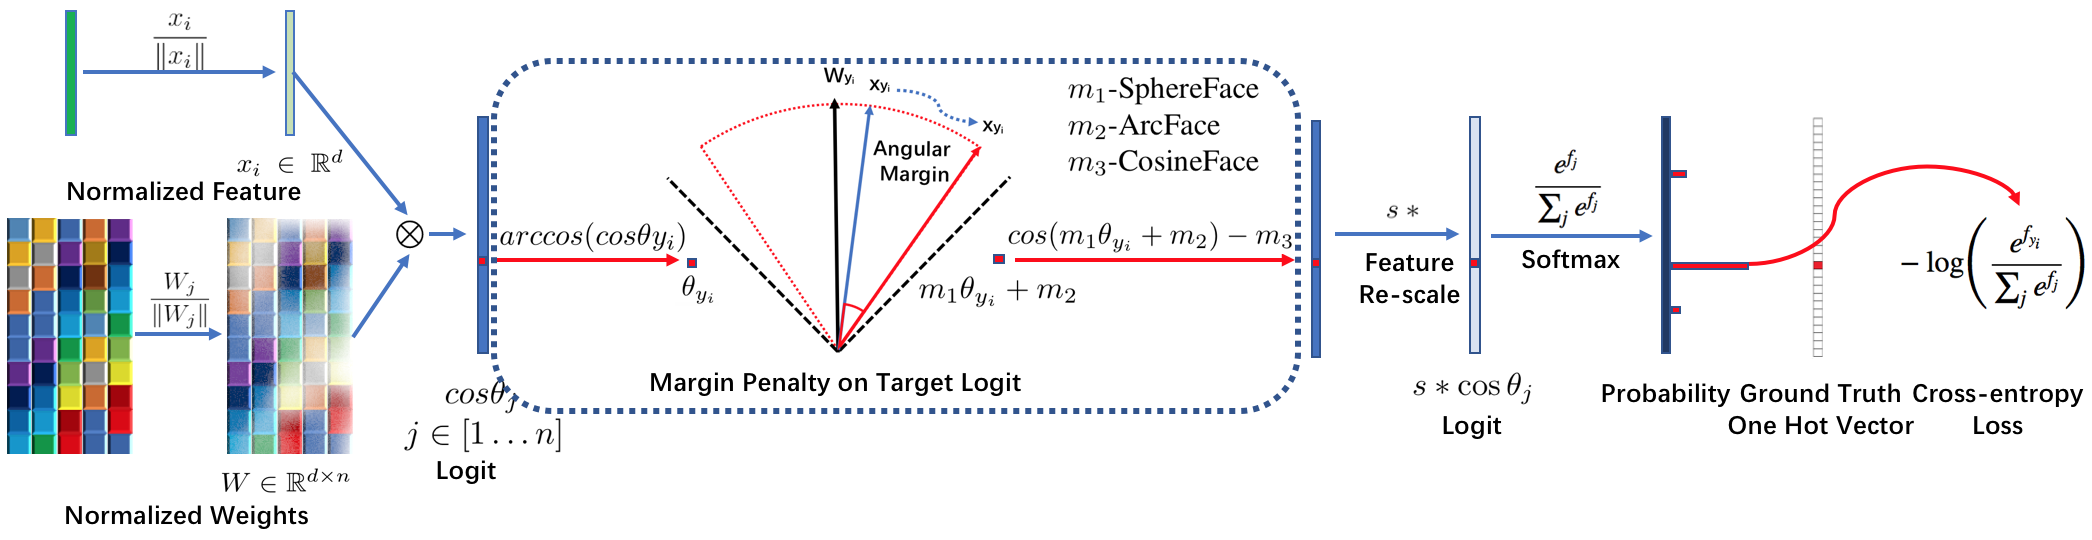
\includegraphics[width=\columnwidth]{images/arcface/arcface.png}
    \caption{Training a CNN for face recognition supervised by the ArcFace loss~\cite{ArcFace}}
    \label{fig:arcface}
\end{figure}

At this point the loss function equation is as follows:
\begin{equation}
    \mathcal{L} = -\frac{1}{N} \sum_{i=1}^{N} \log \frac{e^{s \cos(\theta_{y_i,i})}}
    {e^{s\ \cos(\theta_{y_i,i})} + \sum_{j = 1, j \neq y_i}^n e^{s\ \cos(\theta_{j,i})}}.
\end{equation}

\begin{enumerate}
    \setcounter{enumi}{4}
    \item In the last step the additive angular margin penalty \textit{m} between $x_i$ and $W_{y_i}$ is incorporated.
    The margin is equal to the geodesic distance\footnote{Distance of a curve representing shortest path
    between two points in a surface.} on the hypersphere.
    This is the reason why the method is called \textit{ArcFace}.
\end{enumerate}

Final ArcFace loss function is defined as:
\begin{equation}
    \mathcal{L} = -\frac{1}{N} \sum_{i=1}^{N} \log \frac{e^{s \cos(\theta_{y_i,i} + m)}}
    {e^{s\ \cos(\theta_{y_i,i} + m)} + \sum_{j = 1, j \neq y_i}^n e^{s\ \cos(\theta_{j,i})}}.
\end{equation}
It has been experimentally determined that the best performance is achieved for $m=0.5$.

\section{Comparison with Other Losses}\label{sec:arc-comparison}
By having a look at table~\ref{tbl:arcfaceboundcomp} and figure~\ref{fig:arcfacecomp} we can do a comparison of
geometric differences of different decision margins.

\begin{table}[H]
    \begin{tabularx}{\textwidth}{l|Y}
        Loss Functions & Decision Boundaries \\ \hline
        Softmax~\ref{sec:sphereface-loss} & $\left( W_1 - W_2 \right)x + b_1 - b_2 = 0$ \\
        SphereFace~\ref{sec:sphereface-loss} & $\norm{x} \left( \cos{m\theta_1} - \cos{\theta_2} \right) = 0$ \\
        CosFace~\ref{sec:cosface} & $s \left( \cos{\theta_1} - m - \cos{\theta_2} \right) = 0$ \\
        ArcFace & $s \left( \cos(\theta_1 + m) - \cos{\theta_2} \right) = 0$
    \end{tabularx}
    \caption{Comparison of the decision boundaries under the binary classification case}
    \label{tbl:arcfaceboundcomp}
\end{table}

The advantage of \textit{ArcFace} is its constant linear angular margin throughout the whole interval.

\begin{figure}[H]
    \centering
    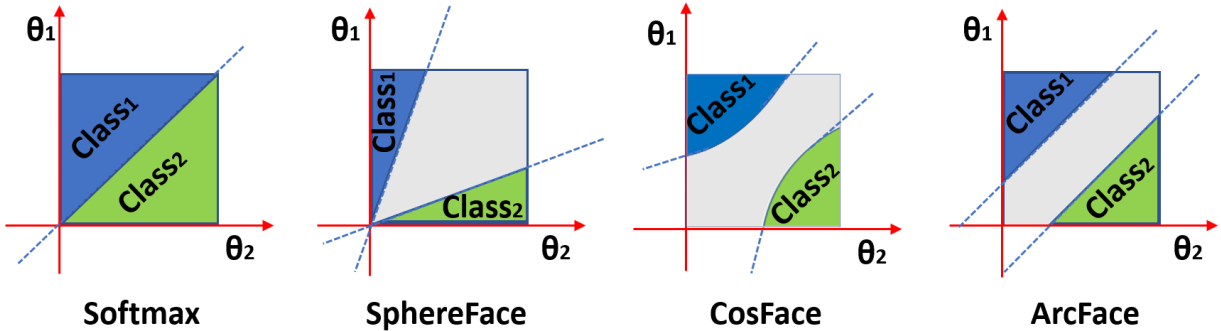
\includegraphics[width=\columnwidth]{images/arcface/arcfacecomparison.png}
    \caption{Decision margins of different loss functions under binary classification case.~\cite{ArcFace}}
    \label{fig:arcfacecomp}
\end{figure}

We can see the concrete percentual results in table~\ref{tbl:arcfacecomp}.
The performance of ResNet100 with ArcFace loss trained on MS1MV2~\ref{subsec:ms1m} dataset exceeded that of other
methods mentioned in this thesis.

\begin{table}[H]
    \begin{tabularx}{\textwidth}{l|XXc}
        Method                & \#Image & LFW~\ref{subsec:lfw}            & YTF~\ref{subsec:ytf}            \\ \hline
        FaceNet~\ref{subsec:facenet}               & 200M    & 99.63          & 95.10          \\
        Center Loss~\ref{sec:center-loss}           & 0.7M    & 99.28          & 94.90          \\
        SphereFace~\ref{sec:sphereface-loss}            & 0.5M    & 99.42          & 95.00          \\
        CosFace~\ref{sec:cosface}               & 5M      & 99.73          & 97.60          \\
        MS1MV2~\ref{subsec:ms1m}, R100, ArcFace & 5.8M    & \textbf{99.83} & \textbf{98.02}
    \end{tabularx}
    \caption{Verification performance (\%) of different methods on LFW and YTF datasets.}
    \label{tbl:arcfacecomp}
\end{table}